\begin{question}
\noindent On a Valorant esports tournament overlay, a designer uses a coordinate grid to animate a map icon. Triangle $J$ is translated to give triangle $K$, as shown on the grid below.

\begin{center}
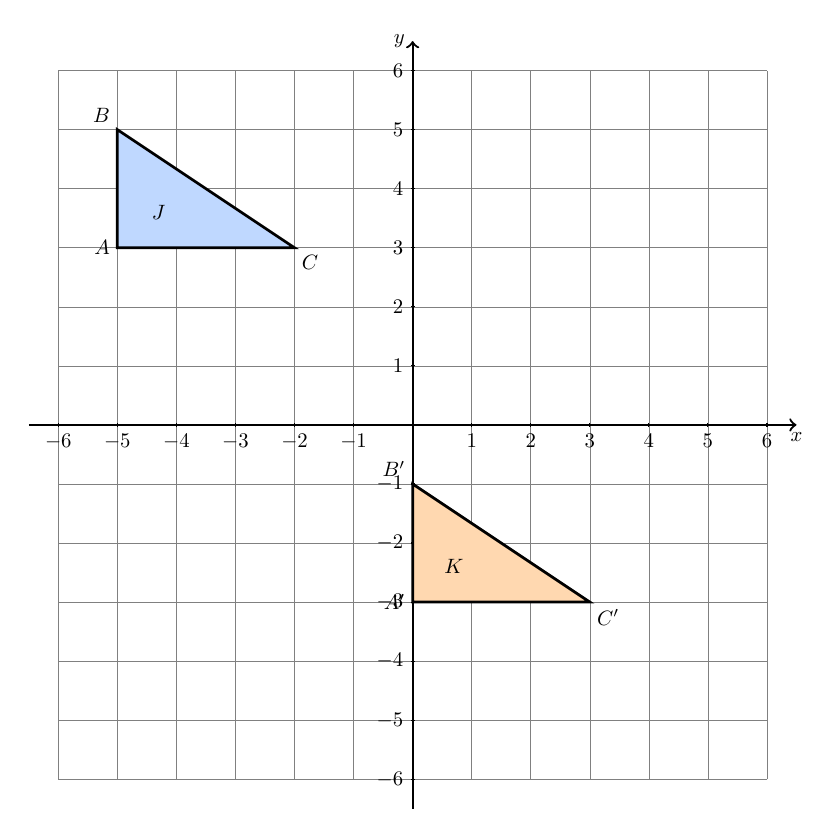
\begin{tikzpicture}[scale=0.75, transform shape]
    \definecolor{borderColour}{HTML}{000000}
    \definecolor{fillColourJ}{HTML}{BFD8FF}
    \definecolor{fillColourK}{HTML}{FFD8B0}

    \def\axisLimit{6}

    % Draw grid
    \draw[step=1cm,gray,very thin] (-\axisLimit,-\axisLimit) grid (\axisLimit,\axisLimit);

    % Draw axes
    \draw[thick,->] (-\axisLimit-0.5,0) -- (\axisLimit+0.5,0) node[anchor=north] {$x$};
    \draw[thick,->] (0,-\axisLimit-0.5) -- (0,\axisLimit+0.5) node[anchor=east] {$y$};

    % Label x-axis and y-axis
    \foreach \x in {-\axisLimit,...,-1,1,2,...,\axisLimit}
        \draw (\x cm,1pt) -- (\x cm,-1pt) node[anchor=north] {$\x$};
    \foreach \y in {-\axisLimit,...,-1,1,2,...,\axisLimit}
        \draw (1pt,\y cm) -- (-1pt,\y cm) node[anchor=east] {$\y$};

    % Triangle J: A(-5,3), B(-5,5), C(-2,3)
    \coordinate (A) at (-5,3);
    \coordinate (B) at (-5,5);
    \coordinate (C) at (-2,3);
    \filldraw[fill=fillColourJ, draw=borderColour, line width=1pt] (A) -- (B) -- (C) -- cycle;
    \node[left] at (A) {$A$};
    \node[above left] at (B) {$B$};
    \node[below right] at (C) {$C$};
    \node at (-4.3,3.6) {$J$};

    % Triangle K: A'(0,-3), B'(0,-1), C'(3,-3)  -- translation vector (5,-6)
    \coordinate (Ap) at (0,-3);
    \coordinate (Bp) at (0,-1);
    \coordinate (Cp) at (3,-3);
    \filldraw[fill=fillColourK, draw=borderColour, line width=1pt] (Ap) -- (Bp) -- (Cp) -- cycle;
    \node[left] at (Ap) {$A'$};
    \node[above left] at (Bp) {$B'$};
    \node[below right] at (Cp) {$C'$};
    \node at (0.7,-2.4) {$K$};

\end{tikzpicture}
\end{center}

\noindent Describe fully the translation that maps triangle $J$ onto triangle $K$.

\vspace{4cm}

\begin{flushright}
    \answerplain{2}
\end{flushright}
\end{question}
